\documentclass[11pt,a4paper,titlepage]{article}

\usepackage[utf8]{inputenc}
\usepackage[english]{babel}
\usepackage{algpseudocode} 
\usepackage{algorithm}
\usepackage{amsmath,amssymb,graphicx,listings,stmaryrd}
\usepackage{tcolorbox}
\usepackage{subcaption}

\algnewcommand{\LineComment}[1]{\State \(\triangleright\) #1}
\algnewcommand\True{\textbf{true}\space}
\algnewcommand\False{\textbf{false}\space}

\newtheorem{definition}{Definition}[section]
 
\usepackage[linkcolor=black,colorlinks=true,citecolor=black,filecolor=black]{hyperref}

\usepackage{xcolor}
\usepackage{tikz}
\usetikzlibrary{arrows, automata}

\newcommand\eqdef{\mathrel{\overset{\makebox[0pt]{\mbox{\normalfont\tiny\sffamily def}}}{=}}}

\setlength{\parindent}{0pt}

\title{Proving Temporal Properties by Abstract Interpretation}
\date{September 6, 2017}
\author{Samuel Marco Ueltschi}


\begin{document}

\maketitle

\tableofcontents
\clearpage

\section{Introduction}
 
Motivation etc.

This section introduces the necessary background for understanding the main concepts described in this thesis.
Note that we assume that the reader already has a basic understanding of abstract interpretation. An detailed introduction into 
the theory of abstract interpretation can be found in [TODO].


\section{State Transition Systems}

To be able to analyse the behaviour of a program, it is necessary 
to express said behavior through a mathematical model. 
We model the operational semantics of programs using transition systems. 
This is based on the definitions presented in~\cite{UrbanM-VMCAI15}.

\begin{definition}{Transition System}
    A transition system is a tuple $\langle \Sigma, \tau \rangle$ where $\Sigma$ 
    is the set of all states in the system and $\tau \in \Sigma \times \Sigma$ 
    is the so called transition relations that defines how one can transition from one state to the other.
\end{definition}

Transition systems allow us to model the semantics of a program 
independently of the programming language in which it was written. 
By expressing the possible transition between states in terms of a relation, 
it is also possible to capture nondeterminism. Figure~\ref{fig:basic_transition_system} 
shows a simple transition system represented as directed graphs. States are represented as nodes
and state transitions as directed edges.
\\

\begin{figure}
\centering
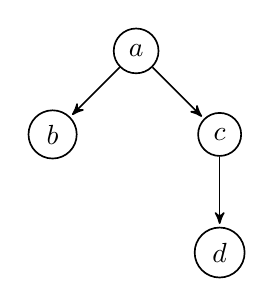
\begin{tikzpicture}[->,>=stealth',shorten >=1pt,auto,node distance=1.5cm,semithick]
    \tikzset{every state/.style={minimum size=0pt}}

    \node[state] (A)                    {$a$};
    \node[state] (B) [below left of=A] {$b$};
    \node[state] (C) [below right of=A]  {$c$};
    \node[state] (D) [below of=C] {$d$};

    \path (A) edge              node {} (B);
    \path (A) edge              node {} (C);
    \path (C) edge              node {} (D);
\end{tikzpicture}
\caption{A basic state transition system} 
\label{fig:basic_transition_system}
\end{figure}


We introduce the following auxiliary functions over states of a transition systems which will become 
useful in section (TODO ref XY) where we defined the semantics of CTL operators in terms of transition systems.

\begin{definition}\label{def:pre}
    Given a transition system $\langle \Sigma, \tau \rangle$. $\text{pre} \colon \mathcal{P}(\Sigma) \to \mathcal{P}(\Sigma)$
    maps a set of states $X \in \mathcal{P}(\Sigma)$ to the set of their predecessors with respect to the program transition
    relation $\tau$:
\begin{equation}
    \text{pre}(X) \eqdef \{s \in \Sigma \ | \ \exists s' \in X \colon \langle s, s' \rangle \in \tau \}  
\end{equation}
\end{definition}


\begin{definition}\label{def:tilde_pre}
    Given a transition system $\langle \Sigma, \tau \rangle$. $\widetilde{\text{pre}} \colon \mathcal{P}(\Sigma) \to \mathcal{P}(\Sigma)$
    maps a set of states $X \in \mathcal{P}(\Sigma)$ to the set of their predecessors with respect to the program transition
    relation $\tau$ with the limitation that only those predecessor states are selected which exclusively transition to states in $X$:
\begin{equation}
    \widetilde{\text{pre}}(X) \eqdef \{s \in \Sigma \ | \ \forall s' \in X \colon \langle s, s' \rangle \in \tau \Rightarrow s' \in X \}  
\end{equation}
\end{definition}

To get an intuition for the difference between $\widetilde{\text{pre}}$ and $\text{pre}$, consider the state transition system 
depicted in figure~\ref{fig:basic_transition_system}. There it holds that $\text{pre}(\{b, d\}) = \{a, c\}$ 
because $a$ is the predecessor of $b$ and $c$ the predecessor of $d$. 
However note that $\widetilde{\text{pre}}(\{b, d\}) = \{c\}$ since only $c$ has 
transitions that exclusively end up in either $b$ or $d$. 
Consequently it holds that $\widetilde{\text{pre}}(\{b, c\}) = \{a\}$ because $a$ transitions exclusively to either $b$ or $c$.


\section{Computation Tree Logic (CTL)}\label{sec:computation_tree_logic}

Computation Tree Logic (CTL) is a logic which allows us to state properties about possible execution traces of state transition systems. 
In the context of this thesis, CTL is used to express temporal properties about the runtime behaviour of programs. 
This section gives a brief introduction into the syntax and semantic of CTL. 
Further information about CTL can be found in~\cite{baier2008principles}.

\subsection{Syntax}
The syntax of a CTL formula is given by the following grammar definition.

\begin{align*}
    \Phi  ::= \ & \\ 
    & a \ | \\
    & \neg \Phi \ | \ \Phi \land \Phi \ | \ \Phi \lor \Phi \ | \\
    & \forall\bigcirc\Phi \ | \ \exists\bigcirc\Phi \ | \\
    & \forall\lozenge\Phi \ | \ \exists\lozenge\Phi \ | \\
    & \forall\square\Phi \ | \ \exists\square\Phi \ | \\
    & \forall(\Phi \ U \ \Phi) | \ \exists(\Phi \ U \ \Phi) 
\end{align*}

The term $a$ is a placeholder for arbitrary atomic propositions.

\subsection{Semantic}

We now define the satisfaction relation $\models$ between states $\sigma \in \Sigma$ and CTL formulae.
The satisfaction relation for atomic propositions depends on the semantics of the underlying 
logic for atomic propositions.

\begin{align*}
    \sigma \models \neg \Phi  &\iff \text{not} \ \sigma \models \Phi \\ 
    \sigma \models \Phi_1 \land \Phi_2   &\iff (\sigma \models \Phi_1) \ \text{and} \ (\sigma \models \Phi_1) \\ 
    \sigma \models \Phi_1 \lor \Phi_2   &\iff (\sigma \models \Phi_1) \ \text{or} \ (\sigma \models \Phi_1) \\ 
    \sigma \models \forall\bigcirc\Phi &\iff \ \forall \pi \in Paths(\sigma) \colon (\pi [1] \models \Phi) \\ 
    \sigma \models \exists\bigcirc\Phi &\iff \ \exists \pi \in Paths(\sigma) \colon (\pi [1] \models \Phi) \\ 
    \sigma \models \forall(\Phi_1 \ U \ \Phi_2) &\iff \ \forall \pi \in Paths(\sigma) \colon 
    (\exists j \geq 0 \colon \pi[j] \models \Phi_2 \land (\forall 0 \leq k < j \colon \pi[k] \models \Phi_1)) \\ 
    \sigma \models \exists(\Phi_1 \ U \ \Phi_2) &\iff \ \exists \pi \in Paths(\sigma) \colon 
    (\exists j \geq 0 \colon \pi[j] \models \Phi_2 \land (\forall 0 \leq k < j \colon \pi[k] \models \Phi_1)) \\ 
    \sigma \models \forall\square\Phi &\iff \ \forall \pi \in Paths(\sigma) \colon (\forall j \geq 0 \colon \pi[j] \models \Phi) \\ 
    \sigma \models \exists\square\Phi &\iff \ \exists \pi \in Paths(\sigma) \colon (\forall j \geq 0 \colon \pi[j] \models \Phi) \\ 
\end{align*}

The states $\sigma \in \Sigma$ are part of a state transition system $\langle \Sigma, \tau \rangle$ and 
$Paths(\sigma_0)$ is the set of all paths $\pi = \sigma_0 \sigma_1 \sigma_2 \dots$ starting from $\sigma_0$ with $\pi[j] = \sigma_j$.
The CTL formulae $\forall\lozenge\Phi$ and $\exists\lozenge\Phi$ are not defined for $\models$ as they are equivalent to 
$\forall(true \ U \ \Phi)$ and $\exists(true \ U \ \Phi)$. Furthermore the following useful equivalence relations 
exists which can be used to relate existential to universal CTL formulae.

\begin{align*}
    \exists\bigcirc\Phi &\equiv \neg \forall\bigcirc(\neg \Phi)\\ 
    \exists\lozenge\Phi &\equiv \neg \forall\square(\neg \Phi) \\
    \exists\square\Phi  &\equiv \neg \forall\lozenge(\neg \Phi) \\
\end{align*}

\subsection{Recurrence and Guarantee Properties}
TODO


\section{Ranking Functions}

The traditional approach for proving termination is based on inferring \textit{ranking functions}~\cite{Touring49}~\cite{Floyd67}.
A ranking function is a partial function from program states to a well-ordered set (e.g.\ the natural numbers). 
To prove termination, the values of the ranking functions must decrease during program execution. Therefore the value that a \textit{ranking function} assigns to a state is an upper bound on the number of steps until the program terminates.
Cousot and Cousot prove the existence of a \textit{most precise ranking function} then can be derived 
by abstract interpretation \cite{CousotCousot-POPL12}. The theory of abstract interpretation makes it possible to express 
various aspects of the semantics of a program. In that context the \textit{most precise ranking function} for termination is called
the \textit{termination semantics}.

\begin{definition}
    The \textit{termination semantics} is a ranking function 
    $\tau^{t} \in \Sigma \rightarrow \mathbb{N}$.
    A program starting from some state $\sigma \in \Sigma$ terminates if and only if $\sigma \in dom(\tau^{t})$.
\end{definition}

By definition of the \textit{termination semantics}, a program will terminate if its initial state is in the domain of
the ranking function. In other words, if the termination semantics assigns a natural value to the initial state that
is an upper bound on the number of steps until termination.\\

Based on the work of Cousot and Cousot~\cite{CousotCousot-POPL12}. Urban and Miné~\cite{UrbanM-VMCAI15} extended the 
\textit{termination semantics} to the more general notion of guarantee properties. A guarantee property states that
some state satisfying a given property is guaranteed to be reached eventually. Termination is therefore just a 
guarantee property stating that some final state will be reached eventually. As for termination, 
the \textit{guarantee semantics} is a ranking function that assigns each state an upper bound on the number of steps
until a state satisfying the given property is reached.

\begin{definition}
    The \textit{guarantee semantics} is a ranking function 
    $\tau_{[S]}^{g} \in \Sigma \rightarrow \mathbb{N}$
    where $S \subseteq \Sigma$ is a set of states satisfying a desired property.
    A program starting from some state $\sigma \in \Sigma$ will reach a state 
    $s \in S$ if and only if $\sigma \in dom(\tau_{[S]}^{g})$.
\end{definition}

In addition to guarantee properties, Urban and Miné~\cite{UrbanM-VMCAI15} also introduced the \textit{recurrence semantics}.
A recurrence property guarantees that a program starting from some state $\sigma \in \Sigma$ will reach some state satisfying
a given property infinitely often. The value assigned to a state by the \textit{recurrence semantics}
is an upper bound on the number of executions steps until a state satisfying the property is reached the next time. 

\begin{definition}
    The \textit{recurrence semantics} is a ranking function 
    $\tau_{[S]}^{r} \in \Sigma \rightarrow \mathbb{N}$
    where $S \subseteq \Sigma$ is a set of states satisfying a desired property.
    A program starting from some state $\sigma \in \Sigma$ will reach a state 
    $s \in S$ infinitely often if and only if $\sigma \in dom(\tau_{[S]}^{r})$.
\end{definition}

Figure \ref{fig:ranking_functios_example} shows an example for the semantics discussed in this section.
We illustrate the ranking functions by labeling the states in the transition systems with the corresponding value assigned to them by the ranking functions. 
The first example (a) shows the \textit{termination semantics} for a state transition system that always terminates. Therefore the initial state
has the value $2$ assigned to it stating that this program terminates in at most two steps.\\

The second example (b) shows the \textit{guarantee semantics} for the guarantee property that states that a gray state will be reached eventually.
This holds for example (b) therefore the initial state has the value $2$ assigned to it. The program reaches a gray state in at most two steps.\\

The last example (c) shows the \textit{recurrence semantics} for the recurrence property that states that a gray state will be reached infinitely often.
As one can see from the transition system, this is not true when starting from the initial state. Therefore the \textit{recurrence semantics} is undefined
for the initial state. However the property would hold when starting from state $c$ or $d$. 
Accordingly these two states have the values $1$ and $0$ assigned to them.\\

We refer to~\cite{UrbanPhd} for a detailed discussion of the various semantics presented in this session.

\begin{figure}
    \begin{subfigure}[b]{0.32\textwidth}
        \centering
        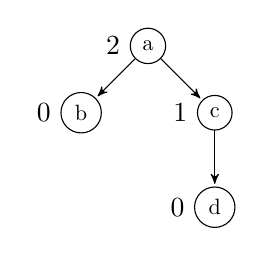
\begin{tikzpicture}[->,>=stealth',shorten >=1pt,node distance=1.5cm,thin]
            \tikzset{every state/.style={minimum size=0pt, scale=0.8}}
            \node[state, label=left:{2}] (A) {a};
            \node[state, label=left:{0}] (B) [below left of=A] {b};
            \node[state, label=left:{1}] (C) [below right of=A] {c};
            \node[state, label=left:{0}] (D) [below of=C] {d};
            \path (A) edge              node {} (B);
            \path (A) edge              node {} (C);
            \path (C) edge              node {} (D);
        \end{tikzpicture}
        \caption{$\tau^{t}$}
    \end{subfigure}
    \begin{subfigure}[b]{0.32\textwidth}
        \centering
        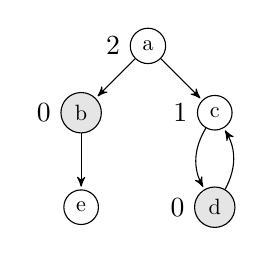
\begin{tikzpicture}[->,>=stealth',shorten >=1pt,node distance=1.5cm,thin]
            \tikzset{every state/.style={minimum size=0pt, scale=0.8}}
            \node[state, label=left:{2}] (A) {a};
            \node[state, fill=gray!20, label=left:{0}] (B) [below left of=A] {b};
            \node[state, label=left:{1}] (C) [below right of=A] {c};
            \node[state, fill=gray!20, label=left:{0}] (D) [below of=C] {d};
            \node[state] (E) [below of=B] {e};
            \path (A) edge              node {} (B);
            \path (A) edge              node {} (C);
            \path (C) edge[bend right]             node {} (D);
            \path (D) edge[bend right]              node {} (C);
            \path (B) edge              node {} (E);
        \end{tikzpicture}
        \caption{$\tau_{[\{b, d\}]}^{g}$}
    \end{subfigure}
    \begin{subfigure}[b]{0.32\textwidth}
        \centering
        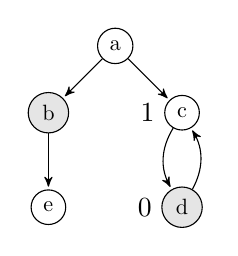
\begin{tikzpicture}[->,>=stealth',shorten >=1pt,node distance=1.5cm,thin]
            \tikzset{every state/.style={minimum size=0pt, scale=0.8}}
            \node[state] (A) {a};
            \node[state, fill=gray!20] (B) [below left of=A] {b};
            \node[state, label=left:{1}] (C) [below right of=A] {c};
            \node[state, fill=gray!20, label=left:{0}] (D) [below of=C] {d};
            \node[state] (E) [below of=B] {e};
            \path (A) edge              node {} (B);
            \path (A) edge              node {} (C);
            \path (C) edge[bend right]             node {} (D);
            \path (D) edge[bend right]              node {} (C);
            \path (B) edge              node {} (E);
        \end{tikzpicture}
        \caption{$\tau_{[\{b, d\}]}^{r}$}
    \end{subfigure}
    \caption{
        Example \textit{termination\ semantics} (a), 
        \textit{guarantee\ semantics} (b) and
        \textit{recurrence\ semantics} (c)
    } 
    \label{fig:ranking_functios_example}
\end{figure}



\section{Concrete Semantics for CTL}\label{sec:ctl_semantics}
In section XY (TODO ref) we introduced the concept of ranking functions and explained how they express the semantics of 
recurrence and guarantee properties. To be able to analyse CTL properties, we extend the notion of ranking functions 
to CTL. Urban et al.~\cite{UrbanM-VMCAI15} define ranking functions for guarantee and recurrence properties.
The CTL semantics presented here are an extension of this work. We will define the \textit{CTL semantics} inductively 
for each CTL operator such that arbitrary combinations of CTL properties can be analyzed. 

\begin{definition}
    The \textit{CTL semantics} for a given CTL formula $\Phi$ is a ranking function 
    $\tau_{\Phi} \in \Sigma \rightarrow \mathbb{N}$. 
    It encodes the semantics of $\Phi$ for a given state transition 
    system $\langle \Sigma, \tau \rangle$ such that $\sigma \models \Phi \iff \sigma \in dom(\tau_{\Phi})$ holds. 
\end{definition}

We start by defining the \textit{CTL semantics} for atomic propositions and logic operators (see definition ~\ref{def:ctl_semantics_basic}).
These definitions follow directly from the satisfiability relation for CTL properties (see section~\ref{sec:computation_tree_logic}). 

\begin{definition}\label{def:ctl_semantics_basic}
    Equations for basic CTL operators
    \setlength{\jot}{15pt}
    \begin{align}
        \tau_a &\eqdef \lambda \sigma.
        \begin{cases}
            0                   & \text{if} \ \sigma \models a \\
            \text{undefined}    & \text{otherwise}
        \end{cases}\\
        %
        \tau_{\neg \Phi} &\eqdef \lambda \sigma.
        \begin{cases}
            0                   & \text{if} \ \sigma \notin dom(\tau_{\Phi}) \\
            \text{undefined}    & \text{otherwise}
        \end{cases}\label{eq:ctl_not}
        \\
        %
        \tau_{\Phi_1 \land \Phi_2} &\eqdef \lambda \sigma.
        \begin{cases}
            \sup\{\tau_{\Phi_1}(s), \tau_{\Phi_2}(\sigma)\} 
                                &\text{if } \sigma \in dom(\tau_{\Phi_1}) \cap dom(\tau_{\Phi_2}) \\
            \text{undefined}    & \text{otherwise}
        \end{cases}\\
        %
        \tau_{\Phi_1 \lor \Phi_2} &\eqdef \lambda \sigma.
        \begin{cases}
            \sup\{\tau_{\Phi_1}(\sigma), \tau_{\Phi_2}(\sigma)\}         & \text{if} \ \sigma \in dom(\tau_{\Phi_1}) \cap dom(\tau_{\Phi_2}) \\
            \tau_{\Phi_1}(\sigma)                                        & \text{if} \ \sigma \in dom(\tau_{\Phi_1}) \setminus dom(\tau_{\Phi_2}) \\
            \tau_{\Phi_2}(\sigma)                                        & \text{if} \ \sigma \in dom(\tau_{\Phi_2}) \setminus dom(\tau_{\Phi_1}) \\
            \text{undefined}    & \text{otherwise}
        \end{cases}
    \end{align}
\end{definition}


Definition~\ref{def:ctl_semantics_until} defines how ranking functions are computed for universal and existential `until' properties.  
This definition is an generalization of the \textit{guarantee semantics} presented in~\cite{UrbanM-VMCAI15}.\\

Recall that for the CTL property $\forall(\Phi_1 U \Phi_2)$ to hold for some state $\sigma \in \Sigma$, 
all paths starting from said state must be a chain of states satisfying $\Phi_1$ ending in a state satisfying $Phi_2$.
We compute $\tau_{\forall(\Phi_1 U \Phi_2)}$ through a least fixed point iteration starting from the totally undefined 
ranking function $\overset{.}{\emptyset}$. The first iteration assigns the value $0$ to all states that satisfy $\Phi_2$. 
In subsequent iterations we consider all states that satisfy $\Phi_1$ and from which one can only transition to states that already satisfy  
$\forall(\Phi_1 U \Phi_2)$. These states are then assigned the largest ranking value of all reachable states plus one. 
By performing iterations this way, we backtrack paths in the state transition systems that end in a state satisfying $\Phi_2$ and which are preceded by an 
unbroken chain of states satisfying $\Phi_1$. Every state on such a path is guaranteed to satisfy the CTL `until' property. 
Furthermore, by starting from $0$ at states that satisfy $\Phi_2$ and increasing while backtracking, 
we are constructing a ranking function in such a way that the value assigned to each state is an 
upper bound on the number of steps until a state is reached that satisfies $\Phi_2$.\\

The $\widetilde{pre}$ relation guarantees that during the backtracking, only those states are considered which 
exclusively transition to states satisfying $\forall(\Phi_1 U \Phi_2)$. 
This condition can be relaxed for existential `until' properties by using the $pre$ relation instead. 
That way, states that have at least one reachable state satisfying $\exists(\Phi_1 U \Phi_2)$ are also considered 
during the backtracking (see definitions~\ref{def:pre} and~\ref{def:tilde_pre}).\\

Figures~\ref{fig:ctl_semantics_universal_until} and~\ref{fig:ctl_semantics_existential_until} give an example on how the
iterative computation for `until' works for universal and existential properties. 
Note how figure~\ref{fig:ctl_semantics_existential_until} has one addition iteration because of the existential quantifier. 
The initial state is added to ranking function in the last iteration because there exists one edge that leads to a state satisfying the property.  
For the universal property, the iteration stops after three iterations because not all successor states
of the initial state satisfy the property.

\begin{definition}\label{def:ctl_semantics_until}
    Equations for CTL until operator
    \setlength{\jot}{15pt}
    \begin{align}
        \tau_{\forall(\Phi_1 U \Phi_2)}  &\eqdef \text{lfp}_{\overset{.}{\emptyset}}^{\sqsubseteq} \ \phi_{\forall(\Phi_1 U \Phi_2)}\\
        \phi_{\forall(\Phi_1 U \Phi_2)}f &\eqdef \lambda \sigma.
        \begin{cases}
            0                                                           
                & \text{if} \ \sigma \in dom(\tau_{\Phi_2}) \\
            \sup\{ f(\sigma') + 1 \ | \ \langle \sigma,\sigma' \rangle \in \tau \}    
                & \text{if} \ \sigma \notin dom(\tau_{\Phi_2}) \ \land \\ 
                & \sigma \in dom(\tau_{\Phi_1}) \ \land \\ 
                & \sigma \in \widetilde{pre}(dom(f)) \\
            \text{undefined}                                            
                & \text{otherwise}
        \end{cases}\\
        \tau_{\exists(\Phi_1 U \Phi_2)}  &\eqdef \text{lfp}_{\overset{.}{\emptyset}}^{\sqsubseteq} \ \phi_{\exists(\Phi_1 U \Phi_2)}\\
        \phi_{\exists(\Phi_1 U \Phi_2)}f &\eqdef \lambda \sigma.
        \begin{cases}
            0                                                           
                & \text{if} \ \sigma \in dom(\tau_{\Phi_2}) \\
            \sup\{ f(\sigma') + 1 \ | \ \langle \sigma,\sigma' \rangle \in \tau \}    
                & \text{if} \ \sigma \notin dom(\tau_{\Phi_2}) \ \land \\ 
                & \sigma \in dom(\tau_{\Phi_1}) \ \land \\ 
                & \sigma \in pre(dom(f)) \\
            \text{undefined}                                            
                & \text{otherwise}
        \end{cases}\\
    \end{align}
\end{definition}

\begin{figure}
    \begin{subfigure}[b]{0.5\textwidth}
        \centering
        \resizebox{100pt}{!}{
            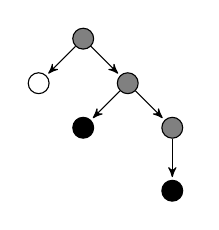
\begin{tikzpicture}[->,>=stealth',shorten >=1pt,auto,node distance=1cm,thin]
                \tikzset{every state/.style={minimum size=0pt, scale=0.8}}
                \node[state, fill=gray] (A) {};
                \node[state] (B) [below left of=A] {};
                \node[state, fill=gray] (C) [below right of=A] {};
                \node[state, fill=black] (D) [below left of=C] {};
                \node[state, fill=gray] (E) [below right of=C] {};
                \node[state, fill=black] (F) [below of=E] {};
                \path (A) edge              node {} (B);
                \path (A) edge              node {} (C);
                \path (C) edge              node {} (D);
                \path (C) edge              node {} (E);
                \path (E) edge              node {} (F);
            \end{tikzpicture}
        }
        \caption{Iteration 0}
    \end{subfigure}
    \begin{subfigure}[b]{0.5\textwidth}
        \centering
        \resizebox{100pt}{!}{
            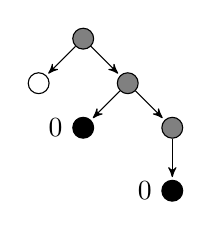
\begin{tikzpicture}[->,>=stealth',shorten >=1pt,auto,node distance=1cm,thin]
                \tikzset{every state/.style={minimum size=0pt, scale=0.8}}

                \node[state, fill=gray] (A) {};
                \node[state] (B) [below left of=A] {};
                \node[state, fill=gray] (C) [below right of=A] {};
                \node[state, fill=black, label=left:{0}] (D) [below left of=C] {};
                \node[state, fill=gray] (E) [below right of=C] {};
                \node[state, fill=black, label=left:{0}] (F) [below of=E] {};

                \path (A) edge              node {} (B);
                \path (A) edge              node {} (C);
                \path (C) edge              node {} (D);
                \path (C) edge              node {} (E);
                \path (E) edge              node {} (F);
            \end{tikzpicture}
        }
        \caption{Iteration 1}
    \end{subfigure}
    \par\bigskip
    \begin{subfigure}[b]{0.5\textwidth}
        \centering
        \resizebox{100pt}{!}{
            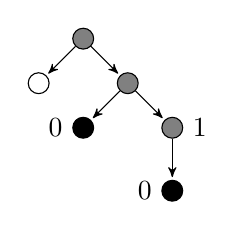
\begin{tikzpicture}[->,>=stealth',shorten >=1pt,auto,node distance=1cm,thin]
                \tikzset{every state/.style={minimum size=0pt, scale=0.8}}

                \node[state, fill=gray] (A) {};
                \node[state] (B) [below left of=A] {};
                \node[state, fill=gray] (C) [below right of=A] {};
                \node[state, fill=black, label=left:{0}] (D) [below left of=C] {};
                \node[state, fill=gray, label=right:{1}] (E) [below right of=C] {};
                \node[state, fill=black, label=left:{0}] (F) [below of=E] {};

                \path (A) edge              node {} (B);
                \path (A) edge              node {} (C);
                \path (C) edge              node {} (D);
                \path (C) edge              node {} (E);
                \path (E) edge              node {} (F);
            \end{tikzpicture}
        }
        \caption{Iteration 2}
    \end{subfigure}
    \begin{subfigure}[b]{0.5\textwidth}
        \centering
        \resizebox{100pt}{!}{
            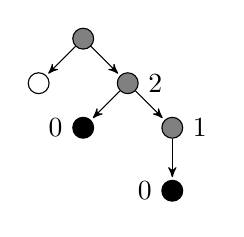
\begin{tikzpicture}[->,>=stealth',shorten >=1pt,auto,node distance=1cm,thin]

                \tikzset{every state/.style={minimum size=0pt, scale=0.8}}

                \node[state, fill=gray] (A) {};
                \node[state] (B) [below left of=A] {};
                \node[state, fill=gray, label=right:{2}] (C) [below right of=A] {};
                \node[state, fill=black, label=left:{0}] (D) [below left of=C] {};
                \node[state, fill=gray, label=right:{1}] (E) [below right of=C] {};
                \node[state, fill=black, label=left:{0}] (F) [below of=E] {};

                \path (A) edge              node {} (B);
                \path (A) edge              node {} (C);
                \path (C) edge              node {} (D);
                \path (C) edge              node {} (E);
                \path (E) edge              node {} (F);
            \end{tikzpicture}
        }
        \caption{Iteration 3}
    \end{subfigure}
    \caption{Iterative computation of $\tau_{\forall(gray \ U \ black)}$.} 
    \label{fig:ctl_semantics_universal_until}
\end{figure}




\begin{figure}
    \begin{subfigure}[b]{0.5\textwidth}
        \centering
        \resizebox{100pt}{!}{
            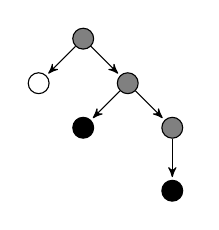
\begin{tikzpicture}[->,>=stealth',shorten >=1pt,auto,node distance=1cm,thin]
                \tikzset{every state/.style={minimum size=0pt, scale=0.8}}
                \node[state, fill=gray] (A) {};
                \node[state] (B) [below left of=A] {};
                \node[state, fill=gray] (C) [below right of=A] {};
                \node[state, fill=black] (D) [below left of=C] {};
                \node[state, fill=gray] (E) [below right of=C] {};
                \node[state, fill=black] (F) [below of=E] {};
                \path (A) edge              node {} (B);
                \path (A) edge              node {} (C);
                \path (C) edge              node {} (D);
                \path (C) edge              node {} (E);
                \path (E) edge              node {} (F);
            \end{tikzpicture}
        }
        \caption{Iteration 0}
    \end{subfigure}
    \begin{subfigure}[b]{0.5\textwidth}
        \centering
        \resizebox{100pt}{!}{
            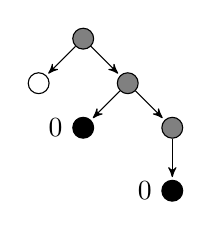
\begin{tikzpicture}[->,>=stealth',shorten >=1pt,auto,node distance=1cm,thin]
                \tikzset{every state/.style={minimum size=0pt, scale=0.8}}

                \node[state, fill=gray] (A) {};
                \node[state] (B) [below left of=A] {};
                \node[state, fill=gray] (C) [below right of=A] {};
                \node[state, fill=black, label=left:{0}] (D) [below left of=C] {};
                \node[state, fill=gray] (E) [below right of=C] {};
                \node[state, fill=black, label=left:{0}] (F) [below of=E] {};

                \path (A) edge              node {} (B);
                \path (A) edge              node {} (C);
                \path (C) edge              node {} (D);
                \path (C) edge              node {} (E);
                \path (E) edge              node {} (F);
            \end{tikzpicture}
        }
        \caption{Iteration 1}
    \end{subfigure}
    \par\bigskip
    \begin{subfigure}[b]{0.32\textwidth}
        \centering
        \resizebox{100pt}{!}{
            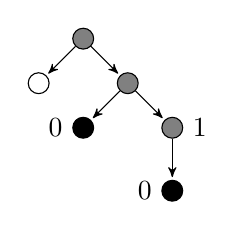
\begin{tikzpicture}[->,>=stealth',shorten >=1pt,auto,node distance=1cm,thin]
                \tikzset{every state/.style={minimum size=0pt, scale=0.8}}

                \node[state, fill=gray] (A) {};
                \node[state] (B) [below left of=A] {};
                \node[state, fill=gray] (C) [below right of=A] {};
                \node[state, fill=black, label=left:{0}] (D) [below left of=C] {};
                \node[state, fill=gray, label=right:{1}] (E) [below right of=C] {};
                \node[state, fill=black, label=left:{0}] (F) [below of=E] {};

                \path (A) edge              node {} (B);
                \path (A) edge              node {} (C);
                \path (C) edge              node {} (D);
                \path (C) edge              node {} (E);
                \path (E) edge              node {} (F);
            \end{tikzpicture}
        }
        \caption{Iteration 2}
    \end{subfigure}
    \begin{subfigure}[b]{0.32\textwidth}
        \centering
        \resizebox{100pt}{!}{
            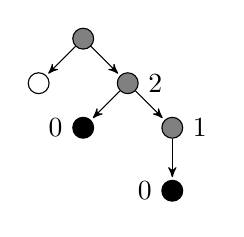
\begin{tikzpicture}[->,>=stealth',shorten >=1pt,auto,node distance=1cm,thin]

                \tikzset{every state/.style={minimum size=0pt, scale=0.8}}

                \node[state, fill=gray] (A) {};
                \node[state] (B) [below left of=A] {};
                \node[state, fill=gray, label=right:{2}] (C) [below right of=A] {};
                \node[state, fill=black, label=left:{0}] (D) [below left of=C] {};
                \node[state, fill=gray, label=right:{1}] (E) [below right of=C] {};
                \node[state, fill=black, label=left:{0}] (F) [below of=E] {};

                \path (A) edge              node {} (B);
                \path (A) edge              node {} (C);
                \path (C) edge              node {} (D);
                \path (C) edge              node {} (E);
                \path (E) edge              node {} (F);
            \end{tikzpicture}
        }
        \caption{Iteration 3}
    \end{subfigure}
    \begin{subfigure}[b]{0.32\textwidth}
        \centering
        \resizebox{100pt}{!}{
            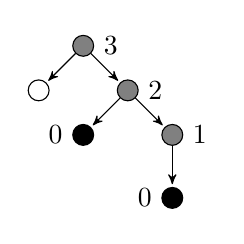
\begin{tikzpicture}[->,>=stealth',shorten >=1pt,auto,node distance=1cm,thin]

                \tikzset{every state/.style={minimum size=0pt, scale=0.8}}

                \node[state, fill=gray, label=right:{3}] (A) {};
                \node[state] (B) [below left of=A] {};
                \node[state, fill=gray, label=right:{2}] (C) [below right of=A] {};
                \node[state, fill=black, label=left:{0}] (D) [below left of=C] {};
                \node[state, fill=gray, label=right:{1}] (E) [below right of=C] {};
                \node[state, fill=black, label=left:{0}] (F) [below of=E] {};

                \path (A) edge              node {} (B);
                \path (A) edge              node {} (C);
                \path (C) edge              node {} (D);
                \path (C) edge              node {} (E);
                \path (E) edge              node {} (F);
            \end{tikzpicture}
        }
        \caption{Iteration 4}
    \end{subfigure}
    \caption{Iterative computation of $\tau_{\exists(gray \ U \ black)}$.} 
    \label{fig:ctl_semantics_existential_until}
\end{figure}


Definition~\ref{def:ctl_semantics_until} defines how ranking functions are computed for universal and existential `global' properties ($\forall\square\Phi$).  
This definition is generalization of the \textit{recurrence semantics} presented in~\cite{UrbanM-VMCAI15}.
The CTL `global' operator states that some property must hold globally for all paths starting from some state in the case of the universal
quantifier ($\forall\square\Phi$) or some path in case of the existential quantifier ($\exists\square\Phi$). 
As for the `until' operator, we distinguish between universal and existential properties by using either $\widetilde{pre}$ or $pre$. 
The ranking function for the `global' operator is computed by greatest fixed point iteration. 
The iteration starts with the ranking function $\tau_\Phi$ of the inner property. 
For each iteration, every state that is still part of the domain of the ranking function is inspected. 
The inspected state is kept in the domain of the ranking function if all its successor states 
(or respectively some for the existential case) are also part of the domain of the ranking function, otherwise it is removed.
The resulting final ranking function is a greatest fixed point that only contains states on paths where the property holds indefinitely.\\

Figures~\ref{fig:ctl_semantics_universal_global} and~\ref{fig:ctl_semantics_existential_global} give an example iteration for 
$\tau_{\exists\square\Phi}$ and $\tau_{\forall\square\Phi}$. Both iterations start with some initial ranking function $\tau_\Phi$.
In the first iteration state `b' is removed because it has no outgoing edges. For the existential case, the iteration stops here because
all remaining states `a', `c' and `'d' have at least one edge to a node thats part of the ranking function. In the universal case we get an additional
iteration that removes state `a' because not all of its successor nodes (namely `b') are part of the ranking function. 

Note that the way $\tau_{\forall\square\Phi}$ and $\tau_{\exists\square\Phi}$ are defined, 
it is not possible to use the `global' operator on finite paths. Only infinite paths are considered to hold globally. 
(TODO state why this choice was made)

\begin{definition}\label{def:ctl_semantics_global}
    Equations for CTL global operator
    \setlength{\jot}{15pt}
    \begin{align}
        \tau_{\forall\square\Phi} &\eqdef \text{gfp}_{\tau_\Phi}^{\sqsubseteq} \  \phi_{\forall\square\Phi}\\
        \phi_{\forall\square\Phi}f &\eqdef \lambda \sigma.
        \begin{cases}
            f(x)                            & \text{if} \ \sigma \in \widetilde{pre}(dom(f)) \\
            \text{undefined}                & \text{otherwise}
        \end{cases}\\
        \tau_{\exists\square\Phi} &\eqdef \text{gfp}_{\tau_\Phi}^{\sqsubseteq} \  \phi_{\exists\square\Phi}\\
        \phi_{\exists\square\Phi}f &\eqdef \lambda \sigma.
        \begin{cases}
            f(x)                            & \text{if} \ \sigma \in pre(dom(f)) \\
            \text{undefined}                & \text{otherwise}
        \end{cases}
    \end{align}
\end{definition}


\begin{figure}

    \begin{subfigure}[b]{0.32\textwidth}
        \centering
        \resizebox{100pt}{!}{
            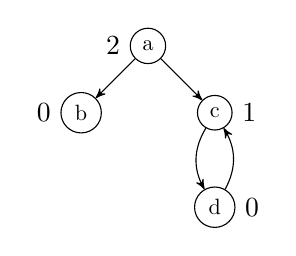
\begin{tikzpicture}[->,>=stealth',node distance=1.5cm,thin]
                \tikzset{every state/.style={minimum size=0pt, scale=0.8}}
                \node[state, label=left:{2}] (A) {a};
                \node[state, label=left:{0}] (B) [below left of=A] {b};
                \node[state, label=right:{1}] (C) [below right of=A] {c};
                \node[state, label=right:{0}] (E) [below of=C] {d};
                \path (A) edge              node {} (B);
                \path (A) edge              node {} (C);
                \path (C) edge[bend right]              node {} (E);
                \path (E) edge[bend right]              node {} (C);
            \end{tikzpicture}
        }
        \caption{Iteration 0}
    \end{subfigure}
    \begin{subfigure}[b]{0.32\textwidth}
        \centering
        \resizebox{100pt}{!}{
            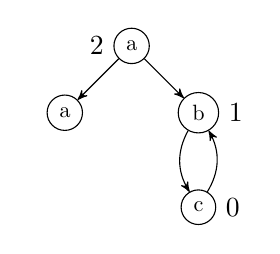
\begin{tikzpicture}[->,>=stealth',node distance=1.5cm,thin]
                \tikzset{every state/.style={minimum size=0pt, scale=0.8}}
                \node[state, label=left:{2}] (A) {a};
                \node[state, label=left:{}] (B) [below left of=A] {a};
                \node[state, label=right:{1}] (C) [below right of=A] {b};
                \node[state, label=right:{0}] (E) [below of=C] {c};
                \path (A) edge              node {} (B);
                \path (A) edge              node {} (C);
                \path (C) edge[bend right]              node {} (E);
                \path (E) edge[bend right]              node {} (C);
            \end{tikzpicture}
        }
        \caption{Iteration 1}
    \end{subfigure}
    \begin{subfigure}[b]{0.32\textwidth}
        \centering
        \resizebox{100pt}{!}{
            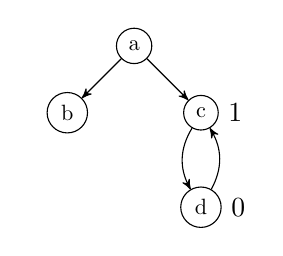
\begin{tikzpicture}[->,>=stealth',node distance=1.5cm,thin]
                \tikzset{every state/.style={minimum size=0pt, scale=0.8}}
                \node[state, label=left:{}] (A) {a};
                \node[state, label=left:{}] (B) [below left of=A] {b};
                \node[state, label=right:{1}] (C) [below right of=A] {c};
                \node[state, label=right:{0}] (E) [below of=C] {d};
                \path (A) edge              node {} (B);
                \path (A) edge              node {} (C);
                \path (C) edge[bend right]              node {} (E);
                \path (E) edge[bend right]              node {} (C);
            \end{tikzpicture}
        }
        \caption{Iteration 2}
    \end{subfigure}
    \caption{Iterative computation of $\tau_{\forall\square\Phi}$.} 
    \label{fig:ctl_semantics_universal_global}
\end{figure}

\begin{figure}
    \begin{subfigure}[b]{0.5\textwidth}
        \centering
        \resizebox{100pt}{!}{
            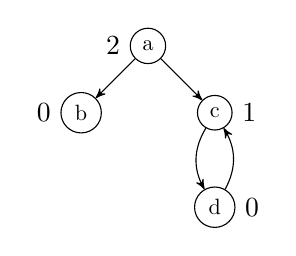
\begin{tikzpicture}[->,>=stealth',node distance=1.5cm,thin]
                \tikzset{every state/.style={minimum size=0pt, scale=0.8}}
                \node[state, label=left:{2}] (A) {a};
                \node[state, label=left:{0}] (B) [below left of=A] {b};
                \node[state, label=right:{1}] (C) [below right of=A] {c};
                \node[state, label=right:{0}] (E) [below of=C] {d};
                \path (A) edge              node {} (B);
                \path (A) edge              node {} (C);
                \path (C) edge[bend right]              node {} (E);
                \path (E) edge[bend right]              node {} (C);
            \end{tikzpicture}
        }
        \caption{Iteration 0}
    \end{subfigure}
    \begin{subfigure}[b]{0.5\textwidth}
        \centering
        \resizebox{100pt}{!}{
            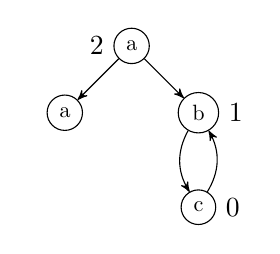
\begin{tikzpicture}[->,>=stealth',node distance=1.5cm,thin]
                \tikzset{every state/.style={minimum size=0pt, scale=0.8}}
                \node[state, label=left:{2}] (A) {a};
                \node[state, label=left:{}] (B) [below left of=A] {a};
                \node[state, label=right:{1}] (C) [below right of=A] {b};
                \node[state, label=right:{0}] (E) [below of=C] {c};
                \path (A) edge              node {} (B);
                \path (A) edge              node {} (C);
                \path (C) edge[bend right]              node {} (E);
                \path (E) edge[bend right]              node {} (C);
            \end{tikzpicture}
        }
        \caption{Iteration 1}
    \end{subfigure}
    \caption{Iterative computation of $\tau_{\exists\square\Phi}$.} 
    \label{fig:ctl_semantics_existential_global}
\end{figure}


Definition~\ref{def:ctl_semantics_next} defines the CTL `next' operator. 
A state satisfies $\forall\bigcirc\Phi$ if all its successors satisfy the property,
correspondingly $\exists\bigcirc\Phi$ is satisfied if at least one successor satisfies the property.
This corresonds to the definition of the $\widetilde{pre}$ and $pre$ relations. Zero is assigned to each state
that satisfies the property. 

\begin{definition}\label{def:ctl_semantics_next}
    Equations for CTL next operator
    \setlength{\jot}{15pt}
    \begin{align}
        \tau_{\forall\bigcirc\Phi} &\eqdef \lambda \sigma.
        \begin{cases}
            0                   & \text{if} \ \sigma \in \widetilde{pre}(dom(\tau_\Phi)) \\
            \text{undefined}    & \text{otherwise}
        \end{cases}\\
        \tau_{\exists\bigcirc\Phi} &\eqdef \lambda \sigma.
        \begin{cases}
            0                   & \text{if} \ \sigma \in pre(dom(\tau_\Phi)) \\
            \text{undefined}    & \text{otherwise}
        \end{cases}
    \end{align}
\end{definition}

\section{Piecewise Defined Ranking Functions}\label{sec:piecewise_defined_ranking_functions}

This section briefly recaps the decision tree abstract domain. 
First we give a description of the domain. 
Then we introduce ordering relations between the elements of the domain 
and relevant operations on the elements of the domain.
An in-depth description of the topics covered in this section can be found in~\cite{UrbanPhd}.  

\subsection{Domain}

The elements of abstract domain are \textit{piecewise-defined} partial functions represented in terms of decision trees. 
The nodes of the trees are linear constrains and the leafs are linear functions. 
Decision trees partition a state space, given by a set of variable $\mathcal{X}$, into linear partitions. 
Each partition is defined through the conjunction of linear constraints on the path from root to leaf in the decision tree.
The linear function at the leaf determines what value is associated to the partition.\\

\begin{figure}
    \centering
    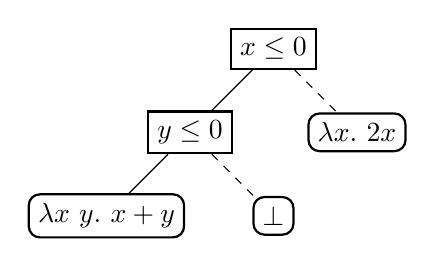
\begin{tikzpicture}[node distance=1.5cm]
        \tikzset{
            inner_node/.style={draw, shape = rectangle, thick},
            leaf/.style={draw, shape = rectangle, rounded corners, thick}
        }
        \node[inner_node] (A) {$x \leq 0$};
        \node[inner_node] (B) [below left of= A] {$y \leq 0$};
        \node[leaf] (C) [below right of= A] {$\lambda x.\ 2x$};
        \node[leaf] (D) [below left of= B] {$\lambda x \ y. \ x + y$};
        \node[leaf] (E) [below right of= B] {$\bot$};
        \path (A) edge              node {} (B);
        \path (A) edge [dashed]              node {} (C);
        \path (B) edge               node {} (D);
        \path (B) edge [dashed]              node {} (E);
    \end{tikzpicture}
    \caption{Example for decision tree}
    \label{fig:decision_tree_example}
\end{figure}


Figure~\ref{fig:decision_tree_example} gives an example for such a decision tree. 
It consists of two nodes with linear constraints $x \leq 0$ and $y \leq 0$. The left most leaf is the function $\lambda x \ y. \ x + y$. 
It is defined for all states satisfying $x \leq 0 \land y \leq 0$ according to the constraints from root to leaf. 
The right most leaf is the function $\lambda x.\ 2x$, it is defined for all states satisfying $\neg (x \leq 0)$ 
(taking a right turn negates the linear constraint of a node). The leaf in the middle is a bottom node, 
signifying that the function for the corresponding partition is undefined. Combining all constraints and functions of
the decision tree in figure~\ref{fig:decision_tree_example} yields the following partial function:

\[
    f(x, y) = \begin{cases}
            x+y                   & \text{if} \ x \leq 0 \land y \leq 0 \\
            2x                   & \text{if} \ x > 0 \\
            \text{undefined}    & \text{otherwise}
        \end{cases}
\]


Now we formalize the domain using mathematical notations.\\

The constrains at the inner nodes of the decision tree are elements of the 
\textit{linear constraints auxiliary abstract domain} $\mathcal{C}$.  

\[
    \mathcal{C} \eqdef 
    \left
        \{ 
        c_1 X_1 + \dots + c_n X_n + c_{n+1} \geq 0 \
        \middle\vert 
        \begin{array}{l}
            \mathcal{X} = \{X_1, \dots, X_n\}\\
            c_1, \dots, c_n, c_{n+1} \in \mathbb{Z} \\
            gcd(|c_1|, \dots, |c_n|, |c_{n+1}|) = 1
        \end{array}
    \right
    \}
\]

The constraints of $\mathcal{C}$ can be instances of the \textit{interval abstract domain}, 
the \textit{octagon abstract domain} or the \textit{polyhedra abstract domain} (TODO cite).\\

Leafs of the decision trees are elements of the \textit{functions auxiliary abstract domain} $\mathcal{F}$.
Elements of $\mathcal{F}$ are either natural valued functions or one of the two special elements $\top_{\mathcal{F}}$ or $\bot_{\mathcal{F}}$.

\[
    \mathcal{F} \eqdef \{ \mathbb{Z}^{|\mathcal{X}|} \rightarrow \mathbb{N} \} \cup \{ \top_{\mathcal{F}}, \ \bot_{\mathcal{F}} \}
\]

We now define the \textit{computational order} $\sqsubseteq_{\mathcal{F}}$ and \textit{approximation order} $\preceq_{\mathcal{F}}$ over
the elements of $\mathcal{F}$.  Intuitively, these partial orders approximate the \textit{computational order} $\sqsubseteq$ 
and \textit{approximation order} $\preceq$ presented in section XY (TODO ref).

In the \textit{computational order} $\sqsubseteq_{\mathcal{F}}$ the special elements $\top_{\mathcal{F}}$ and $\bot_{\mathcal{F}}$
are comparable whereas in the \textit{approximation order} $\preceq_{\mathcal{F}}$ they are incomparable as shown in the 
Hasse diagrams in figure~\ref{fig:function_comp_approx_hasse}. 
Regular function elements are compared point wise.

\[
    f_1 \sqsubseteq_{\mathcal{F}} f_2  \iff  f_1 \preceq_{\mathcal{F}} f_2 \iff
    \forall x \in \mathbb{Z}^{|\mathcal{X}|} \colon f_1(x) \leq f_2(x)
\]


\begin{figure}
    \begin{subfigure}[b]{0.5\textwidth}
        \centering
        \begin{tikzpicture}[]
            \node (top) at (0,2) {$\top_{\mathcal{F}}$};
            \node (f) at (0,1) {$f \colon  \mathbb{Z}^{|\mathcal{X}|} \rightarrow \mathbb{N} $};
            \node (bot) at (0,0) {$\bot_{\mathcal{F}}$};
            \draw (top) -- (f) -- (bot);
        \end{tikzpicture}
        \caption{\textit{computational order} $\sqsubseteq_{\mathcal{F}}$}
    \end{subfigure}
    \begin{subfigure}[b]{0.5\textwidth}
        \centering
        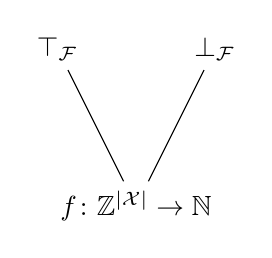
\begin{tikzpicture}[]
            \node (top) at (0,2) {$\top_{\mathcal{F}}$};
            \node (bot) at (2,2) {$\bot_{\mathcal{F}}$};
            \node (f) at (1,0) {$f \colon  \mathbb{Z}^{|\mathcal{X}|} \rightarrow \mathbb{N} $};
            \draw (top) -- (f) -- (bot);
        \end{tikzpicture}
        \caption{\textit{approximation order} $\preceq_{\mathcal{F}}$}
    \end{subfigure}
    \caption{Hasse diagrams for $\sqsubseteq_{\mathcal{F}}$ and $\preceq_{\mathcal{F}}$
    } 
    \label{fig:function_comp_approx_hasse}
\end{figure}

We now define the decision tree abstract domain $\mathcal{T}$.
An element $t \in \mathcal{T}$ is either a \textit{leaf node} $LEAF \colon f$ consisting of a function $f \in \mathcal{F}$ (denoted $t.f$),
or a \textit{decision node} $NODE\{c\}: l; r$ consists of a linear constraint $c \in \mathcal{C}$ (denoted $t.c$) 
and a left and a right sub tree $l, r \in \mathcal{T}$ 
(denoted $t.l$ and $t.r$).
\[
    \mathcal{T} \eqdef \{LEAF \colon f \ | \ f \in \mathcal{F}\} \cup \{NODE\{c\}: l; r \ | \ c \in \mathcal{C}, l, r \in \mathcal{T} \} 
\]


For algorithmic purposes we also define $\mathcal{T}_{NIL}$. 
This adds an additional leaf element $NIL$ to $\mathcal{T}$ to represent the absence of information about a partition. 
\[
    \mathcal{T}_{NIL} \eqdef \{NIL\} \ \cup \ \{LEAF \colon f \ | \ f \in \mathcal{F}\} \ \cup \ \{NODE\{c\}: l; r \ | \ c \in \mathcal{C}, l, r \in \mathcal{T}_{NIL}  \} 
\]


\subsection{Unification}
The function $tree\_unification \colon (\mathcal{T}_{NIL} \times \mathcal{T}_{NIL}) \rightarrow (\mathcal{T}_{NIL} \times \mathcal{T}_{NIL})$ takes two trees
as input and reshapes them such that they have the same inner node structure i.e.\ the same linear constraints. 
The resulting trees are semantically equivalent to their original. This simplifies comparing the partitions of two trees to each other.
The $tree\_unification$ algorithm is described in great detail in~\cite{UrbanPhd}.


\begin{algorithm}                      
    \caption{Tree Join Helper}         
    \label{alg:tree_join_helper}       
    \begin{algorithmic}
        \LineComment{$t_{left}, t_{right} \in \mathcal{T}$}
        \LineComment{$f_{LEAF} \in \mathcal{P}(\mathcal{C}) \rightarrow \mathcal{F} \rightarrow \mathcal{F} \rightarrow \mathcal{T} $}
        \LineComment{$f_{LeftNIL}, f_{RightNIL} \in \mathcal{P}(\mathcal{C}) \rightarrow \mathcal{F} \rightarrow \mathcal{T} $}
        \Function{tree\_join\_helper}{$t_{left}, t_{right}, f_{LEAF}, f_{LeftNIL}, f_{RightNIL}$} 

        \Function{aux}{$t_l, t_r, C$} 

        \If{$isNil(t_l) \land isNil(t_r)$}
            \State \Return $NIL$
        \ElsIf{$isNil(t_l) \land isLeaf(t_r)$}
            \State \Return $f_{LeftNIL}(C, t_r.f)$
        \ElsIf{$isLeaf(t_l) \land isNil(t_r)$}
            \State \Return $f_{RightNIL}(C, t_l.f)$
        \ElsIf{$isLeaf(t_l) \land isLeaf(t_r)$}
            \State \Return $f_{LEAF}(C, t_l.f t_r.f)$
        \Else
            \Comment{assert $t_l.c = t_r.c$}
            \State $l \gets \Call{aux}{t_l.l, t_r.l,  \{t_l.c\} \cup C}$
            \State $r \gets \Call{aux}{t_l.r, t_r.r, \{\neg t_l.c\} \cup C}$
            \State \Return $LEAF\{t_l.c\} \colon l ; r $
        \EndIf

        \EndFunction

        \State $(t_l, t_r) \gets \Call{tree\_unification}{t_{left}, t_{right}}$
        \State \Return \Call{aux}{$t_l, t_r$}
        \EndFunction
\end{algorithmic}
\end{algorithm}



\subsection{Join}\label{sec:tree_join}
Two trees can be joined to form the union of all partitions represented by the trees. There are two variations of the join operator. 
The \textit{computational join} $\sqcup_{\mathcal{T}} \colon (\mathcal{T}_{NIL} \times \mathcal{T}_{NIL}) \rightarrow \mathcal{T}_{NIL}$
and the \textit{approximation join} $\curlyvee_{\mathcal{T}} \colon (\mathcal{T}_{NIL} \times \mathcal{T}_{NIL}) \rightarrow \mathcal{T}_{NIL}$. 
The first one joins leaf nodes with $\sqsubseteq_{\mathcal{F}}$ the latter with $\preceq_{\mathcal{F}}$. Figure~\ref{fig:decision_tree_join_example} 
demonstrates the difference between the two join types. When joining two trees where one defines a function for a 
partition and the other does not (see left leaf in $t_1$ and $t_2$), the \textit{computational join} will preserve the defined function
and the \textit{approximation join} will set the partition to undefined. For detailed discussion about the two join types see~\cite{UrbanPhd}.

\begin{figure}
    \begin{subfigure}[b]{0.5\textwidth}
        \centering
        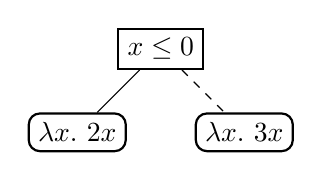
\begin{tikzpicture}[node distance=1.5cm]
            \tikzset{
                inner_node/.style={draw, shape = rectangle, thick},
                leaf/.style={draw, shape = rectangle, rounded corners, thick}
            }
            \node[inner_node] (A) {$x \leq 0$};
            \node[leaf] (B) [below left of= A] {$\lambda x.\ 2x$};
            \node[leaf] (C) [below right of= A] {$\lambda x. \ 3x$};

            \path (A) edge              node {} (B);
            \path (A) edge [dashed]              node {} (C);
        \end{tikzpicture}
        \caption{$t_1$}
    \end{subfigure}
    \begin{subfigure}[b]{0.5\textwidth}
        \centering
        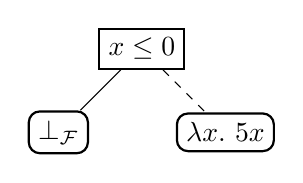
\begin{tikzpicture}[node distance=1.5cm]
            \tikzset{
                inner_node/.style={draw, shape = rectangle, thick},
                leaf/.style={draw, shape = rectangle, rounded corners, thick}
            }
            \node[inner_node] (A) {$x \leq 0$};
            \node[leaf] (B) [below left of= A] {$\bot_{\mathcal{F}}$};
            \node[leaf] (C) [below right of= A] {$\lambda x. \ 5x$};
            \path (A) edge              node {} (B);
            \path (A) edge [dashed]              node {} (C);
        \end{tikzpicture}
        \caption{$t_2$}
    \end{subfigure}
    \par\bigskip
    \begin{subfigure}[b]{0.5\textwidth}
        \centering
        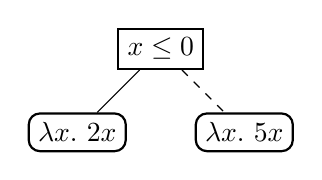
\begin{tikzpicture}[node distance=1.5cm]
            \tikzset{
                inner_node/.style={draw, shape = rectangle, thick},
                leaf/.style={draw, shape = rectangle, rounded corners, thick}
            }
            \node[inner_node] (A) {$x \leq 0$};
            \node[leaf] (B) [below left of= A] {$\lambda x.\ 2x$};
            \node[leaf] (C) [below right of= A] {$\lambda x. \ 5x$};
            \path (A) edge              node {} (B);
            \path (A) edge [dashed]              node {} (C);
        \end{tikzpicture}
        \caption{$t_1 \sqcup_{\mathcal{T}} t_2$}
    \end{subfigure}
    \begin{subfigure}[b]{0.5\textwidth}
        \centering
        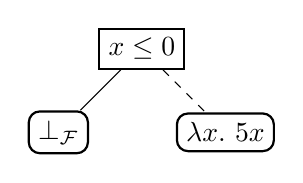
\begin{tikzpicture}[node distance=1.5cm]
            \tikzset{
                inner_node/.style={draw, shape = rectangle, thick},
                leaf/.style={draw, shape = rectangle, rounded corners, thick}
            }
            \node[inner_node] (A) {$x \leq 0$};
            \node[leaf] (B) [below left of= A] {$\bot_{\mathcal{F}}$};
            \node[leaf] (C) [below right of= A] {$\lambda x. \ 5x$};

            \path (A) edge              node {} (B);
            \path (A) edge [dashed]              node {} (C);
        \end{tikzpicture}
        \caption{$t_1 \curlyvee_{\mathcal{T}} t_2$}
    \end{subfigure}

    \caption{Decision Tree Join Example}
    \label{fig:decision_tree_join_example}
\end{figure}

\subsection{Meet}\label{sec:tree_meet}

\subsection{Filter}
TODO

\subsection{Reset}
TODO

\subsection{Backward Assign}
TODO


\section{Abstract Semantics for CTL}

In this section we present a sound, computable abstraction of the CTL semantics $\tau_\Phi$.\\

Computing the ranking function $\tau_\Phi$ is in general not computable as one can easily encode the 
halting problem in $\tau_\Phi$. Therefore, we settle for a sound but computable approximation of $\tau_\Phi$ by using
the abstract domain of piecewise defined ranking functions presented in section~\ref{sec:piecewise_defined_ranking_functions}.

\begin{definition}
    The abstract CTL semantics $\tau^{\sharp}_\Phi \in \mathcal{L} \rightarrow \mathcal{T}$ is a sound approximation of the
    CTL semantics $\tau_\Phi$ with regards to the \textit{approximation order} $\preceq$.
\end{definition}

Recall that the CTL semantics $\tau_\Phi \in \Sigma \rightarrow \mathbb{N}$ is a partial function that 
assigns numerical values to program states $\sigma \in \Sigma$. 
In the abstract version, program states are partitioned by decision trees $t \in \mathcal{T}$ and 
grouped by program labels $l \in \mathcal{L}$. A program satisfies a given CTL property $\Phi$ if the decision tree of the
initial program label $\tau^{\sharp}_\Phi(t_{init})$ is defined over all partitions 
(TODO introduce notion of defined w.r.t decision trees).
\\

The following sections present how to compute $\tau^{\sharp}_\Phi$ for each CTL operator. 
We start with the basic operators $\land, \lor, \neg$ and atomic propositions that can be computed directly 
from the control-flow-graph (CFG). 
Then we present how to compute the universal $\forall U$, $\forall\bigcirc$ and $\forall\square$ operators through fixed point iteration. 
Followed by a discussion on how to adapt the universal operators to their existential version.

\subsection{Atomic Propositions}

Atomic propositions are path independent, therefore abstract CTL semantics $\tau^{\sharp}_a$ assigns the same decision tree to 
each program label $l \in \mathcal{L}$. The decision tree assigns the constant value $0$ to all partitions that satisfy the atomic proposition.
We compute this by using the $\text{RESET} \llbracket a \rrbracket$ operator on the totally undefined decision tree $\bot$ (see section XY TODO). 

\begin{definition}\label{def:abstract_ctl_semantics_atomic}
    Abstract CTL semantics for atomic propositions
    \begin{align}
        \tau^{\sharp}_{a} \eqdef \ \lambda l. \ \text{RESET} \llbracket a \rrbracket \bot
    \end{align}
\end{definition}


\begin{tcolorbox}
    \subsubsection*{Fixing the \text{RESET} operator}
    The $\text{RESET}\llbracket a \rrbracket$ operator was originally introduced in~\cite{UrbanPhd} in the context of abstract guarantee semantics
    and would overapproximate the set of partitions that satisfy the atomic proposition $a$. 
    During the work on this thesis, we discovered that this original definition is actually unsound and leads to incorrect analysis results. \\
    
    The problem is best described using an example. Consider the abstract CTL semantics $\tau^{\sharp}_{x^2 < y^3 + 1}$. 
    The non linear constraint $x^2 < y^3 + 1$ can usually not be represented by any of the common numerical domains. 
    An overapproximating implementation of $\text{RESET}\llbracket x^2 < y^3 + 1 \rrbracket$ will therefore
    reset some pairs $(x, y)$ for which $x^2 < y^3 + 1$ does not hold which is unsound as to the definition of
    the CTL semantics $\tau_{x^2 < y^3 + 1}$. Note that this problem propagates to more complex temporal properties that
    depend on atomic propositions.\\

    We resolve this problem by using an underapproximating implementation of $\text{RESET}$ as presented
    in section XY (TODO ref).
\end{tcolorbox}


\subsection{Logical Operators}
In this section we define the logical operators $\land$, $\lor$ and $\neg$ for the abstract CTL semantics.
All of the mentioned operators will are defined inductively over the abstract CTL semantics of the nested properties in
definition~\ref{def:abstract_ctl_semantics_logic_operators}.

\begin{definition}\label{def:abstract_ctl_semantics_logic_operators}
    Abstract CTL semantics for logic operators
    \begin{align}
        \tau^{\sharp}_{\Phi_1 \land \Phi_2} &\eqdef \ \lambda l. \ (\tau^{\sharp}_{\neg \Phi_1}l) \ \sqcup_{\mathcal{T}} \ (\tau^{\sharp}_{\neg \Phi_2}l)
        \label{eq:abstract_ctl_and}\\
        \tau^{\sharp}_{\Phi_1 \lor \Phi_2} &\eqdef \ \lambda l. \ (\tau^{\sharp}_{\neg \Phi_1}l) \ \sqcap_{\mathcal{T}} \ (\tau^{\sharp}_{\neg \Phi_2}l)
        \label{eq:abstract_ctl_or}\\
        \tau^{\sharp}_{\neg \Phi} &\eqdef \ \lambda l. \ \text{COMPLEMENT} \ (\tau^{\sharp}_{\neg \Phi}l)
        \label{eq:abstract_ctl_not}
    \end{align}
\end{definition}

The abstract CTL semantics for $\land$ and $\lor$ (equations~\ref{eq:abstract_ctl_and} and~\ref{eq:abstract_ctl_or}) combine the decision trees
of the nested properties piecewise for each program label.\\

The \textit{computational join} $\sqcup_{\mathcal{T}}$ is used to combine the two trees (see section~\ref{sec:tree_join}) in
case of the logical $\lor$. This operator forms the union of the two decision trees. 
Note that we use the computational version of the join operator to include partitions that are defined in at least one of the two trees. 
If a partition is defined in both trees, the smallest upper bound of the assigned value is formed to approximate the concrete CTL semantics.\\

The corresponding definition for the logical $\land$ operator forms the intersection of the two trees by using the
\textit{computational meet} $\sqcap_{\mathcal{T}}$ (see section~\ref{sec:tree_meet}). 
As with the logical $\lor$, the smallest upper bound is formed if a partition is defined for both trees. 
By using the computational version of the operator, we ensure that no $NIL$ leafs are introduced.\\

For the logical $\neg$ operator we introduce the new $\text{COMPLEMENT}$ operator which, 
in a nutshell, forms the complement of a ranking function represented by a decision tree. 
The $\text{COMPLEMENT}$ operator is implemented in algorithm (TODO ref).

Every state that was originally defined in the tree will become undefined and vice-versa.

However one has to be careful when forming the complement of a decision tree. Decision trees are an 
approximation of the concrete CTL semantics. Therefore not all states that are undefined in the abstract decision tree
are actually undefined in the concrete. Partitions that are undefined because of this uncertainty are marked with a $\top$
leaf. These leafs have to be ignored when forming the complement of a decision tree.   





\subsection{Universal Operators}
\subsection{Existential Operators}







\pagebreak

\bibliographystyle{IEEEbib}
\bibliography{bibl_conf}



\end{document}
